\documentclass[border=2pt]{standalone}
\usepackage{amsmath,amssymb}
\usepackage{tikz}
\usetikzlibrary{arrows.meta,positioning,fit,calc}
\usepackage{mathptmx}
\definecolor{teal}{HTML}{0F766E}
\definecolor{tealbg}{HTML}{ECF7F5}
\definecolor{inkgray}{HTML}{4B5563}
\begin{document}
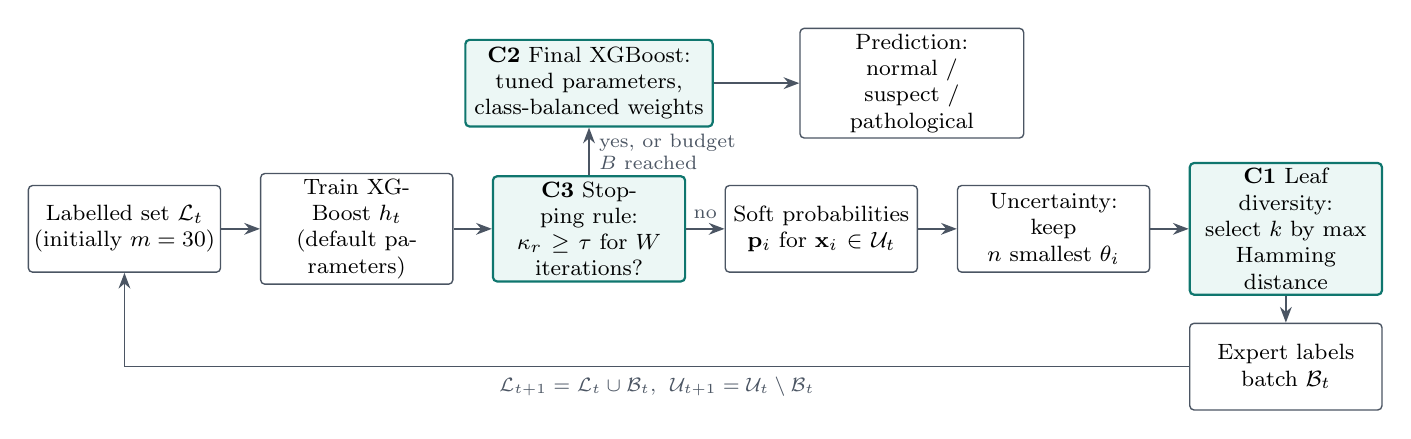
\begin{tikzpicture}[
  font=\footnotesize, >={Stealth[length=2mm]},
  box/.style={draw=inkgray, line width=0.5pt, rounded corners=1.5pt, align=center, minimum height=11mm, text width=23mm, inner sep=2pt, fill=white},
  key/.style={box, draw=teal, line width=0.8pt, fill=tealbg},
  arr/.style={->, line width=0.6pt, draw=inkgray},
  lab/.style={font=\scriptsize, text=inkgray}]
\node[box] (L) at (0,0) {Labelled set $\mathcal{L}_t$\\ (initially $m=30$)};
\node[box] (X) at (2.95,0) {Train XGBoost $h_t$\\ (default parameters)};
\node[key] (S) at (5.9,0) {\textbf{C3} Stopping rule:\\ $\kappa_r\ge\tau$ for $W$\\ iterations?};
\node[box] (P) at (8.85,0) {Soft probabilities\\ $\mathbf{p}_i$ for $\mathbf{x}_i\in\mathcal{U}_t$};
\node[box] (U) at (11.8,0) {Uncertainty: keep\\ $n$ smallest $\theta_i$};
\node[key] (D) at (14.75,0) {\textbf{C1} Leaf diversity:\\ select $k$ by max\\ Hamming distance};
\node[box] (O) at (14.75,-1.75) {Expert labels\\ batch $\mathcal{B}_t$};
\node[key, text width=30mm] (F) at (5.9,1.85) {\textbf{C2} Final XGBoost:\\ tuned parameters,\\ class-balanced weights};
\node[box, text width=27mm] (Y) at (10.0,1.85) {Prediction: normal /\\ suspect / pathological};
\draw[arr] (L) -- (X); \draw[arr] (X) -- (S);
\draw[arr] (S) -- node[lab, above]{no} (P);
\draw[arr] (P) -- (U); \draw[arr] (U) -- (D); \draw[arr] (D) -- (O);
\draw[arr] (O.west) -- node[lab, below]{$\mathcal{L}_{t+1}=\mathcal{L}_t\cup\mathcal{B}_t$,\; $\mathcal{U}_{t+1}=\mathcal{U}_t\setminus\mathcal{B}_t$} (0,-1.75) -- (L.south);
\draw[arr] (S) -- node[lab, right, align=left]{yes, or budget\\ $B$ reached} (F);
\draw[arr] (F) -- (Y);
\end{tikzpicture}
\end{document}
